% Unofficial University of Cambridge Poster Template
% https://github.com/andiac/gemini-cam
% a fork of https://github.com/anishathalye/gemini
% also refer to https://github.com/k4rtik/uchicago-poster

\documentclass[final]{beamer}

% ====================
% Packages
% ====================

\usepackage[T1]{fontenc}
\usepackage{lmodern}
\usepackage[orientation=landscape,size=a0,scale=1.0]{beamerposter}
\usetheme{gemini}
\usecolortheme{nott}
\usepackage{graphicx}
\usepackage{booktabs}
\usepackage{tikz}
\usepackage{pgfplots}
\pgfplotsset{compat=1.14}
\usepackage{anyfontsize}
\usepackage{wrapfig} % Required for text wrapping

% ====================
% Lengths
% ====================

% If you have N columns, choose \sepwidth and \colwidth such that
% (N+1)*\sepwidth + N*\colwidth = \paperwidth
\newlength{\sepwidth}
\newlength{\colwidth}
\setlength{\sepwidth}{0.025\paperwidth}
\setlength{\colwidth}{0.45\paperwidth}

\newcommand{\separatorcolumn}{\begin{column}{\sepwidth}\end{column}}

% ====================
% Title
% ====================

\title{Global Land Ice Measurements From Space}

\author{Andrew P. Barrett \inst{1} \and Robyn Marowitz \inst{1} \and Donna Scott \inst{1}}

\institute[shortinst]{\inst{1} National Snow and Ice Data Center, CIRES, University of Colorado Boulder}

% ====================
% Footer (optional)
% ====================

\footercontent{
  \href{https://www.glims.org}{https://www.glims.org} \hfill
  NSIDC 50th Anniversary \hfill
  \href{mailto:andrew.barrett@colorado.edu}{andrew.barrett@colorado.edu}}
% (can be left out to remove footer)


% ====================
% Logo (optional)
% ====================

% use this to include logos on the left and/or right side of the header:
\logoright{\includegraphics[height=7cm]{logos/nsidc_cires_logo_combined.png}}
\logoleft{\includegraphics[height=7cm]{logos/glims_logo_smooth_small.png}}

% ====================
% Body
% ====================

\begin{document}

% Refer to https://github.com/k4rtik/uchicago-poster
% logo: https://www.cam.ac.uk/brand-resources/about-the-logo/logo-downloads
% \addtobeamertemplate{headline}{}
% {
%     \begin{tikzpicture}[remember picture,overlay]
%       \node [anchor=north west, inner sep=3cm] at ([xshift=-2.5cm,yshift=1.75cm]current page.north west)
%       {\includegraphics[height=7cm]{logos/unott-logo.eps}}; 
%     \end{tikzpicture}
% }

\begin{frame}[t]
\begin{columns}[t]
\separatorcolumn

\begin{column}{\colwidth}

  \begin{block}{What is GLIMS?}

    The Global Land Ice Measurements from Space, GLIMS, is an
    initiative to map and monitor the worlds glaciers using mostly optical
    satellite and aerial imagery.  Glacier outlines are mapped by a
    global collective of glaciologists from academic institutions and
    national and state agencies.  Outlines are archived in the GLIMS Glacier
    Database hosted at NSIDC.

    A \textit{glim} is an archaic Scottish term that means ``a passing look; a glimpse; as much as is seen at a glance''.  Glacier outlines mapped by GLIMS may be seen as a \textit{glim} of a passing or changing phenomenon.

    \begin{figure}[h]
      \centering
      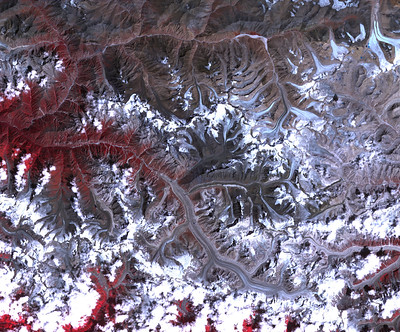
\includegraphics[width=0.6\textwidth]{images/gangotri_aster_20010901_400x332.jpg}
      \caption{Gangotri Glacier, Uttarakhand, India, captured on September 9, 2001, by the Advanced Spaceborne Thermal Emission and Reflection Radiometer (ASTER) sensor on NASA’s Terra satellite.}
      \label{fig:gangotri_aster}
    \end{figure}
        
  \end{block}

  \begin{alertblock}{A History of GLIMS}

    \begin{figure}[h]
      \centering
      \includegraphics[width=0.9\textwidth]{images/glims_history_timeline.png}
      \caption{Time of of evolution of GLIMS initiative and GLIMS at NSIDC}
      \label{fig:timeline}
    \end{figure}

  \end{alertblock}

\end{column}

\separatorcolumn

\begin{column}{\colwidth}

  \begin{block}{Growth of Glacier Outlines in GLIMS}

    \begin{wrapfigure}{r}{0.6\textwidth}
      \centering
      \includegraphics[width=0.58\textwidth]{images/glacier_count_maps_series.png}
      \caption{Number of glacier outlines for various date ranges.  The 1990 to 2010 time period corresponds to the time period used to create the Randolph Glacier Inventory.}
      \label{fig:glacier_count_timeseries}
    \end{wrapfigure}
        

    The GLIMS Glacier Database is a multitemporal geospatial database that contains vector representations of glacier features.  The majority of features in the database are glacier outlines but the database also includes debris covered regions of glaciers, supraglacial and proglacial lakes, seasonal snowlines, and glacier centerlines.

    The earliest outlines, from 1450, are created by mapping moraines.  The database also includes Outlines for the late 19th century that have been mapped from paper maps, mostly in the European Alps.  The bulk of the outlines are mapped from aerial orthoimagery and optical satellite images.  Digital terrain models are also used as additional information.

    Many outlines are mapped by hand.  Mapping is often done using band ratios of multi-spectral data.  Automated or semi-automated mapping methods are also employed.  However, final outlines are often edited by hand.  Machine learning methods are increasingly being used for mapping.
    
  \end{block}


\end{column}
\separatorcolumn



\end{columns}
\end{frame}

\end{document}
